\documentclass[11pt,a4paper]{article}
\usepackage[margin=22mm]{geometry}
\usepackage[T1]{fontenc}
\usepackage{lmodern}
\usepackage{tabularx,booktabs,hyperref,xcolor,array,xurl}
\usepackage{tikz}
\usetikzlibrary{arrows.meta,positioning,fit,shapes.geometric}
\usepackage{enumitem}
\usepackage{listings}
\hypersetup{colorlinks=true,linkcolor=blue,urlcolor=blue,citecolor=blue}
\setlength{\parindent}{0pt}\sloppy
\setlength{\parskip}{6pt}
\renewcommand{\arraystretch}{1.15}
\newcolumntype{Y}{>{\raggedright\arraybackslash}X}
\newcolumntype{P}[1]{>{\raggedright\arraybackslash}p{#1}}
\newcommand{\code}[1]{\nolinkurl{#1}}
\newcommand{\status}[1]{\textbf{#1}}
\title{}
\author{}
\date{}

\begin{document}
\begin{center}
{\Large\textbf{23CSE455 Design Patterns}}\\[4pt]
{\LARGE\textbf{Part 2 Findings: Evolution and Refactoring}}\\[6pt]
{\large Design Pattern Identification and Evolution in a Spring MVC-Based Warehouse Management Application}
\end{center}

\textbf{Team: B9}\\
\textbf{Date: 11 October 2026} (re-audited findings)\\
\textbf{Team working repository:} \href{https://github.com/akdswordguy/Team_B9_DP}{akdswordguy/Team\_B9\_DP}\\
\textbf{Companion documents:} \code{report/main.tex} (full report), \code{report/part1_findings.tex}, \code{report/part3_findings.tex}


\begin{tabularx}{\linewidth}{@{}P{0.25\linewidth}P{0.19\linewidth}P{0.10\linewidth}X@{}}
\toprule
Roll number & Student name & Batch \\
\midrule
AM.SC.U4CSE23215 & D Aditya Kiran & CSE C \\
AM.SC.U4CSE23235 & Mithun Krishna & CSE C \\
AM.SC.U4CSE23248 & Sai Kishen K M & CSE C\\
AM.SC.U4CSE23359 & Sivadev Smijith & CSE D \\
\bottomrule
\end{tabularx}

Evidence paths in this document are relative to \code{Team_B9_Findings/Part2/} in the team working repository unless stated otherwise.

\section{Overview}

\begin{tabularx}{\linewidth}{@{}P{0.22\linewidth}P{0.20\linewidth}YP{0.17\linewidth}@{}}
\toprule
Change & Where & Nature & Tests\\
\midrule
\textbf{CH01 Multiple-Warehouse Support} & Upstream \code{org.openwms.common.service.lib} and \code{org.openwms.common.service} & Uncommitted modification of real OpenWMS repositories & 187 run, 7 skipped (Library); 1 (Service) --- recorded\\
\textbf{CH02 Barcode-Based Picking} & \code{CH02-barcode-picking/} & Standalone Spring Boot reference implementation & 14/14 --- recorded; 14 \code{@Test} in source\\
\textbf{CH03 Automatic Stock Reordering} & \code{CH03-stock-reorder/} & Standalone Spring Boot reference implementation & 19/19 --- recorded; 19 \code{@Test} in source\\
\bottomrule
\end{tabularx}

CH02 and CH03 are reference implementations because the canonical modules were not accessible: the OpenWMS CORE README lists the Picking Library as a private GPLv3 repository and the Inventory Service as private preview. None of the three changes is an upstream merged change, and none introduces a new GoF pattern.

\textbf{Re-audit method (11 October 2026).} CH01 was checked by diffing the published complete-source snapshots against fresh clones of the two upstream repositories at their baselines. CH02 and CH03 were checked by recounting files, physical Java LOC and \code{@Test} methods in the published source, reading every test, and confirming that each acceptance claim matches code. Maven could not be re-run because Maven Central was blocked in the audit environment, so build and test totals marked ``recorded'' are the team's original runs.

\section{CH01 --- Multiple-Warehouse Support}

\subsection{Requirement}
Introduce explicit warehouse identity so that locations with identical coordinates can exist in different warehouses without collision. A location belongs to one warehouse; its identity is the warehouse plus the existing five-part \code{LocationPK} (area, aisle, x, y, z). Coordinate uniqueness is warehouse-scoped; PLC and ERP codes stay globally unique. \code{LocationGroup} remains a logical grouping and does not become a warehouse. An unqualified lookup that matches several warehouses must not silently pick one.

\subsection{Provenance and baselines}
\begin{tabularx}{\linewidth}{@{}P{0.34\linewidth}P{0.36\linewidth}Y@{}}
\toprule
Repository & Baseline commit & CH01 state\\
\midrule
\href{https://github.com/openwms/org.openwms.common.service.lib}{\nolinkurl{openwms/org.openwms.common.service.lib}} & \code{a6566d7a90364f8cb0e82ec013720b644926dffe} & 31 modified, 13 new files; uncommitted\\
\href{https://github.com/openwms/org.openwms.common.service}{\nolinkurl{openwms/org.openwms.common.service}} & \code{fc7edd4ffbe16de65d482b3a2d462d4d896b1998} & 2 modified files; uncommitted\\
\bottomrule
\end{tabularx}

\textbf{Re-audit result.} Diffing \code{CH01-multiple-warehouses/*.complete-source/} against upstream reproduced the changed-file lists in \code{PROVENANCE.md} exactly. The Library grew from 226 to 238 Java files (12 new Java files plus the new \code{9-warehouse.adoc}). The partial evidence snapshots are byte-identical to the complete-source copies, apart from a UTF-8 byte-order mark on one \code{README.md}. Credential-bearing files were excluded from the copies, so the snapshots are source-complete but not guaranteed standalone builds.

\subsection{Design change}
\begin{itemize}[nosep]
\item New \code{org.openwms.common.warehouse} package: \code{Warehouse} entity, \code{WarehouseController}, \code{WarehouseService}/\code{WarehouseServiceImpl}, \code{WarehouseRepository}, \code{WarehouseMapper}, \code{WarehouseApi}, \code{WarehouseVO}.
\item \code{Location} gains a mandatory (\code{nullable = false}) \code{Warehouse} reference, and the \code{UC_LOC_ID} unique constraint changes from (\code{C_AREA}, \code{C_AISLE}, \code{C_X}, \code{C_Y}, \code{C_Z}) to (\code{C_WAREHOUSE}, \code{C_AREA}, \code{C_AISLE}, \code{C_X}, \code{C_Y}, \code{C_Z}). \code{UC_LOC_PLC_CODE} and \code{UC_LOC_ERP_CODE} are unchanged.
\item Location and transport-unit services, controllers, APIs, the \code{LocationMO} message and the command handler gain warehouse-qualified operations; unqualified operations still work when the coordinate is unique and are rejected when it is ambiguous.
\item No default warehouse and no data migration are added.
\end{itemize}

\subsection{Acceptance criteria and test evidence}
The CH01 tests are identifiable by name: 18 test methods were added (245 \code{@Test} annotations at the baseline, 263 after).

\begin{tabularx}{\linewidth}{@{}P{0.22\linewidth}YP{0.15\linewidth}@{}}
\toprule
Criterion & Test methods (class.method) & Status\\
\midrule
Same coordinates in different warehouses & \code{LocationTest.same_coordinates_in_different_warehouses_are_distinct_locations}; \code{LocationIT.shall_allow_same_coordinates_in_different_warehouses}; \code{LocationServiceImplIT.shall_allow_same_location_id_in_different_warehouses_and_find_by_warehouse} & Recorded as passed\\
Duplicate coordinates in one warehouse & None. Enforced by the \code{UC_LOC_ID} constraint only. & Enforced by schema; not tested\\
Warehouse-qualified lookup and update & \code{TransportUnitServiceImplIT.update_with_warehouse_code_selects_the_requested_warehouse_for_duplicate_coordinates}; \code{TransportUnitCommandHandlerIT.creates_transport_units_at_the_same_coordinates_in_the_requested_warehouses} & Recorded as passed\\
Ambiguous unqualified lookup rejected & \code{TransportUnitServiceImplIT.update_without_warehouse_code_rejects_an_ambiguous_coordinate}; \code{TransportUnitCommandHandlerIT.rejects_unqualified_creation_when_the_coordinate_is_ambiguous} & Recorded as passed\\
Unique unqualified lookup still works & \code{TransportUnitServiceImplIT.update_without_warehouse_code_resolves_a_unique_coordinate}; \code{TransportUnitCommandHandlerIT.creates_without_warehouse_when_the_coordinate_is_unique} & Recorded as passed\\
Unknown warehouse rejected & \code{LocationServiceImplIT.shall_reject_location_with_unknown_warehouse}; \code{WarehouseServiceImplIT.rejects_an_unknown_warehouse_code} & Recorded as passed\\
Warehouse management & \code{WarehouseServiceImplIT.creates_and_retrieves_a_warehouse}, \code{rejects_a_duplicate_warehouse_code} & Recorded as passed\\
API/message carry warehouse code & \code{LocationServiceImplIT.location_api_and_message_carry_warehouse_code}; \code{LocationMOTest.warehouse_code_is_preserved_by_json_serialization} & Recorded as passed\\
Legacy \code{LocationMO} constructor & \code{LocationMOTest.legacy_nine_argument_constructor_preserves_null_warehouse} & Recorded as passed\\
PLC/ERP global uniqueness & None. \code{UC_LOC_PLC_CODE}/\code{UC_LOC_ERP_CODE} unchanged from baseline. & Preserved by schema; not tested\\
\code{LocationGroup} semantics & Source/design review. & Preserved by design\\
Production data rollout & No migration/backfill supplied. & Not completed\\
\bottomrule
\end{tabularx}

\subsection{Recorded verification}
\begin{itemize}[nosep]
\item Library: Maven 3.9.9 \code{mvn.cmd -DforkCount=0 install} --- \texttt{BUILD SUCCESS}; 187 tests, 0 failures, 0 errors, 7 skipped. Asciidoctor logged errors for an unavailable generated snippet and invalid part structure despite the successful status.
\item Common Service: \code{mvn.cmd -DforkCount=0 verify} --- \texttt{BUILD SUCCESS}; 1 test, 0 failures/errors/skips; Failsafe reported no integration tests.
\item \code{git diff --check} exited 0 in both CH01 repositories and in CORE.
\end{itemize}

\subsection{Pattern impact, metrics and limitations}
No new GoF pattern is introduced; the Part 1 Observer and Composite instances are untouched, and the generic \code{TreeNode} Composite does not become a warehouse hierarchy. No before/after LOC metrics were recorded and none are estimated. The changes remain uncommitted, so there is no after commit. Because \code{C_WAREHOUSE} is non-nullable, existing production locations need an explicit warehouse assignment before rollout; no Flyway/Liquibase migration or backfill is supplied, and ORM auto-update is not a substitute.

\section{CH02 --- Barcode-Based Picking}

\subsection{Requirement and design}
Resolve a scanned barcode to stock, validate the item and quantity, pick, and return the updated stock.

\textbf{Before} (\code{5ca90cc}): \code{PickingController} $\rightarrow$ \code{PickingService.pickByItemId} $\rightarrow$ \code{StockRepository.findById} $\rightarrow$ \code{StockItem.pick}, exposed as \code{POST /api/picking/item}.

\textbf{After} (\code{0f0fbf0}): \code{PickingController.pickByBarcode} $\rightarrow$ \code{PickingService.pickByBarcode} $\rightarrow$ \code{BarcodeResolver.resolve} $\rightarrow$ \code{StockRepository.findByBarcode}; the service validates quantity, calls \code{StockItem.pick}, saves, and returns a \code{PickingResult}. \code{PickingExceptionHandler} maps \code{InvalidPickingQuantityException} to 400, \code{BarcodeNotFoundException} to 404, and \code{InsufficientStockException}/\code{StockUnavailableException} to 409. \code{PickingRequest} validates \code{@NotBlank barcode} and \code{@Min(1) quantity}. The direct item-ID route is kept.

\begin{center}
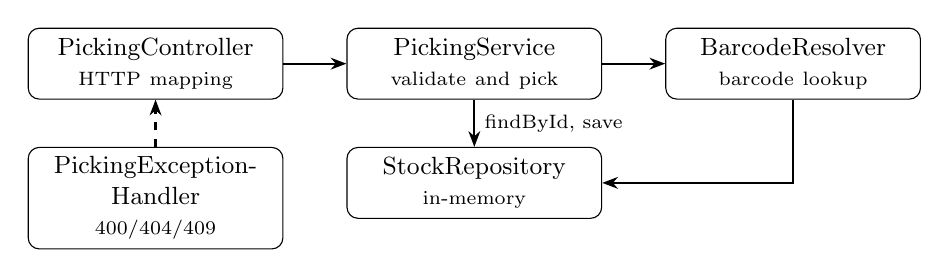
\begin{tikzpicture}[
  node distance=6mm and 8mm,
  box/.style={draw,rounded corners,align=center,text width=30mm,minimum height=9mm,font=\small},
  arr/.style={-{Stealth[length=2mm]},thick}
]
\node[box] (c) {PickingController\\\scriptsize HTTP mapping};
\node[box,right=of c] (s) {PickingService\\\scriptsize validate and pick};
\node[box,right=of s] (b) {BarcodeResolver\\\scriptsize barcode lookup};
\node[box,below=of s] (r) {StockRepository\\\scriptsize in-memory};
\node[box,below=of c] (h) {PickingException\-Handler\\\scriptsize 400/404/409};
\draw[arr] (c)--(s); \draw[arr] (s)--(b); \draw[arr] (b)|-(r); \draw[arr] (s)--node[right,font=\scriptsize]{findById, save}(r);
\draw[arr,dashed] (h)--(c);
\end{tikzpicture}
\end{center}

\subsection{Acceptance criteria and test evidence}
\begin{tabularx}{\linewidth}{@{}P{0.08\linewidth}P{0.26\linewidth}YP{0.08\linewidth}@{}}
\toprule
ID & Criterion & Test methods & Result\\
\midrule
AC1 & Valid barcode resolves and pick succeeds & \code{PickingControllerTest.post_valid_barcode_picks_stock_and_returns_result}; \code{PickingServiceTest.picks_stock_resolved_from_a_barcode_and_decreases_quantity}; \code{BarcodeResolverTest.resolves_an_existing_barcode_to_its_stock_item} & Pass\\
AC2 & Unknown barcode rejected without creating stock & \code{BarcodeResolverTest.rejects_an_unknown_barcode_without_creating_stock}; \code{PickingControllerTest.post_unknown_barcode_returns_not_found} & Pass\\
AC3 & Unavailable stock cannot be picked & \code{PickingServiceTest.rejects_unavailable_stock}; \code{PickingControllerTest.post_unavailable_stock_returns_conflict} & Pass\\
AC4 & Quantity above stock rejected & \code{PickingServiceTest.rejects_quantity_greater_than_available_stock}; \code{PickingControllerTest.post_excessive_quantity_returns_conflict} & Pass\\
AC5 & Successful pick decreases and returns remaining quantity & \code{PickingServiceTest.picks_stock_resolved_from_a_barcode_and_decreases_quantity} & Pass\\
AC6 & Zero and negative quantities rejected & \code{PickingServiceTest.rejects_zero_and_negative_quantities}; \code{PickingControllerTest.post_zero_quantity_returns_bad_request} & Pass\\
AC7 & Direct item-ID picking still works separately & \code{PickingServiceTest.picks_a_requested_quantity_by_stock_item_id}, \code{direct_item_id_picking_remains_available_separately}; \code{PickingControllerTest.direct_item_id_endpoint_remains_separate_and_available} & Pass\\
AC8 & Endpoint returns documented statuses & All six \code{PickingControllerTest} methods (200, 400, 404, 409) & Pass\\
\bottomrule
\end{tabularx}

Recorded: \code{mvn.cmd -DforkCount=0 verify} --- \texttt{BUILD SUCCESS}, 14 tests, 0 failures. The source contains exactly 14 \code{@Test} methods (6 controller, 2 resolver, 6 service). Ignored, generated \code{PickingControllerIT} Surefire files from a deleted test source are stale and excluded.

\subsection{Metrics}
\begin{tabularx}{\linewidth}{@{}Yrrrrr@{}}
\toprule
State & Prod.\ files & Test files & Total files & Java LOC & Tests\\
\midrule
Before (\code{5ca90cc}) & 7 & 1 & 8 & 197 & 1\\
After (\code{0f0fbf0}) & 14 & 3 & 17 & 526 & 14\\
\bottomrule
\end{tabularx}
LOC is physical lines including blanks and comments. The after row was re-measured from the published source and matches. The before row cannot be re-measured from the team repository (Section~5).

\subsection{Pattern impact and limitations}
No new GoF pattern. MVC separation and the repository interface are architectural mechanisms, and \code{BarcodeResolver} is a focused collaborator, not Strategy or Adapter. Storage is an in-memory demo with one seeded item (barcode \code{8901234567890}); there is no database, scanner hardware or external integration.

\section{CH03 --- Automatic Stock Reordering}

\subsection{Requirement and design}
Add per-item reorder rules and automatically create a reorder request when consumption brings stock to or below the threshold. A reorder is created when \code{availableQuantity <= reorderThreshold} and \code{availableQuantity < targetQuantity}; the requested quantity is \code{targetQuantity - availableQuantity}. Rules reject a blank item ID, a negative threshold, and a target not greater than the threshold.

\textbf{Before} (\code{e9ad4c1}): \code{StockController} $\rightarrow$ \code{StockService.consume} $\rightarrow$ \code{StockRepository} $\rightarrow$ \code{StockItem.consume}; no reorders.

\textbf{After} (\code{59b1b59}): after a successful consume, \code{StockService} calls \code{ReorderService.evaluate(itemId)}, which loads stock and rule, returns an existing OPEN request if present, and otherwise creates one when the rule fires. \code{evaluate} and \code{complete} are \code{synchronized}. \code{ReorderController} exposes evaluate (200, or 204 when no reorder is needed), list, get and complete; \code{ReorderRuleController} manages rules. Completing a request adds its quantity back to stock and marks it COMPLETED; completing it again is rejected (409).

\subsection{Acceptance criteria and test evidence}
\begin{tabularx}{\linewidth}{@{}P{0.08\linewidth}P{0.26\linewidth}YP{0.08\linewidth}@{}}
\toprule
ID & Criterion & Test methods & Result\\
\midrule
AC1 & Stock above threshold: no reorder & \code{ReorderRuleTest.stock_above_threshold_does_not_require_reorder}; \code{ReorderServiceTest.stock_above_threshold_does_not_create_a_request} & Pass\\
AC2 & Stock equal to threshold: reorder & \code{ReorderRuleTest.stock_equal_to_threshold_requires_reorder_to_target}; \code{ReorderServiceTest.stock_equal_to_threshold_creates_a_request_for_the_gap_to_target} & Pass\\
AC3 & Stock below threshold: reorder & \code{ReorderRuleTest.stock_below_threshold_calculates_quantity_to_target}; \code{ReorderServiceTest.stock_below_threshold_creates_a_request_for_the_gap_to_target} & Pass\\
AC4 & Quantity = target $-$ available & Same tests as AC2 and AC3 (they assert the gap) & Pass\\
AC5 & OPEN request reused & \code{ReorderServiceTest.repeated_evaluation_reuses_the_open_request} & Pass\\
AC6 & Invalid rules rejected & \code{ReorderRuleTest.rejects_negative_threshold}, \code{rejects_target_that_is_not_greater_than_threshold}; \code{StockReorderControllerTest.invalid_rule_is_rejected} & Pass\\
AC7 & Completion replenishes stock & \code{ReorderServiceTest.automatic_reorder_after_consumption_and_completion_allow_a_future_request}; \code{StockReorderControllerTest.completing_request_replenishes_stock_and_allows_a_later_reorder} & Pass\\
AC8 & Later low stock creates a new request & Same two tests as AC7 & Pass\\
AC9 & Consumption triggers evaluation & \code{StockReorderControllerTest.consuming_stock_automatically_creates_a_reorder_that_can_be_listed}; \code{ReorderServiceTest.automatic_reorder_after_consumption_and_completion_allow_a_future_request} & Pass\\
AC10 & Unknown stock rejected & \code{ReorderServiceTest.unknown_stock_item_is_rejected_when_evaluating}; \code{StockServiceTest.unknown_item_is_rejected}; \code{StockReorderControllerTest.unknown_stock_item_is_not_found} & Pass\\
AC11 & Requests retrievable and listable & \code{ReorderServiceTest.reorder_request_can_be_retrieved_by_id_and_as_a_list} & Pass\\
--- & Repeated completion rejected & \code{ReorderServiceTest.completing_an_already_completed_request_is_rejected} & Pass\\
\bottomrule
\end{tabularx}

Recorded: \code{mvn.cmd -DforkCount=0 verify} --- \texttt{BUILD SUCCESS}, 19 tests, 0 failures. The source contains exactly 19 \code{@Test} methods (\code{ReorderRuleTest} 5, \code{ReorderServiceTest} 8, \code{StockReorderControllerTest} 4, \code{StockServiceTest} 2).

\textbf{Test-quality observation.} \code{StockServiceTest.consumption_reduces_stock_without_creating_a_reorder} configures no rule and asserts only the remaining quantity; it does not check that no request was created. The no-reorder behavior is still covered by the AC1 tests.

\subsection{Metrics}
\begin{tabularx}{\linewidth}{@{}Yrrrrr@{}}
\toprule
State & Prod.\ files & Test files & Total files & Java LOC & Tests\\
\midrule
Before (\code{e9ad4c1}) & 6 & 1 & 7 & 169 & 2\\
After (\code{59b1b59}) & 24 & 4 & 28 & 978 & 19\\
\bottomrule
\end{tabularx}
The after row was re-measured from the published source and matches.

\subsection{Pattern impact and limitations}
No new GoF pattern. \code{ReorderRule} encapsulates one fixed predicate and calculation; with no family of interchangeable algorithms it is not Strategy. Stock, rules, requests and IDs are in memory and lost on restart, and \code{synchronized} only serializes calls inside one process. There is no supplier, purchase-order, ERP or messaging integration.

\section{Commit availability}
The CH02 and CH03 before/after commit IDs (\code{5ca90cc}/\code{0f0fbf0} and \code{e9ad4c1}/\code{59b1b59}) refer to the original local project repositories. Those histories were not copied into the team repository, which contains only the after source trees. As a result, the commits cannot be checked out from the submission, and the before metrics cannot be reproduced from it. Publishing the two project histories (for example as Git bundles or separate repositories) would make them verifiable.

\section{Pattern counts after the evolutions}

\begin{tabularx}{\linewidth}{
    @{}
    >{\raggedright\arraybackslash}p{0.22\linewidth}
    *{4}{>{\centering\arraybackslash}p{0.095\linewidth}}
    >{\raggedright\arraybackslash}X
    @{}
}
\toprule
Snapshot / change & Types & Instances & Concrete classes & Rejected candidates & Notes\\
\midrule
Part 1 baseline & 2 & 2 & 2 & 2 & Observer and generic Composite confirmed.\\
After CH01 & 2 & 2 & 2 & 2 & No new GoF pattern; changes uncommitted.\\
After CH02 & 2 & 2 & 2 & 2 & Separate reference implementation; no new GoF pattern.\\
After CH03 & 2 & 2 & 2 & 2 & Separate reference implementation; no new GoF pattern.\\
\bottomrule
\end{tabularx}

These counts carry the frozen Part 1 inventory forward for consistency; they are not a fresh pattern scan of each reference project.

\section{Corrections made in the re-audit}

\begin{tabularx}{\linewidth}{@{}P{0.24\linewidth}YY@{}}
\toprule
Item & Previously & Now\\
\midrule
CH01 test evidence & ``Exact test names/count not retained.'' & 18 named test methods mapped to criteria.\\
CH01 duplicate coordinates in one warehouse & ``Recorded as passed.'' & Enforced by \code{UC_LOC_ID}; no test exercises it.\\
CH01 PLC/ERP uniqueness & ``Evidence recorded; test mapping incomplete.'' & Constraints unchanged from baseline; not tested.\\
CH03 test evidence & ``Source evidence does not supply individual test method names.'' & All 19 methods named and mapped to AC1--AC11.\\
CH02/CH03 commits & Presented as checkable evidence. & Noted as local history not included in the team repository.\\
CH03 typo & ``textended'' & ``extended''\\
\bottomrule
\end{tabularx}

\section{Evidence files}
\begin{itemize}[nosep]
\item \code{CH01-multiple-warehouses/PROVENANCE.md} --- baselines, changed-file lists, exclusions, recorded verification, re-audit test mapping.
\item \code{CH02-barcode-picking/CH02_EVIDENCE.md}, \code{CH03-stock-reorder/CH03_EVIDENCE.md} --- design, API, criteria, tests, metrics, limitations, re-audit notes.
\item \code{CH03-stock-reorder/CH03-class-diagram.puml} --- CH03 class relationships.
\item \code{Team_B9_Findings/LLM_RECORDS/LLM_RECORDS.md} --- records CH01-01, CH01-02, the CH01 verification addendum, CH02-01, CH03-01 and AUDIT-01.
\end{itemize}

\end{document}
